\section{Introduction partielle}
$ _{} $ $ _{} $ $ _{} $ $ _{} $ $ _{} $Dans les chapitres précédents, nous avons esquissé tout l'environnement du système que nous avons prévu élaborer à travers ce mémoire. A présent, nous allons présenter avec précision les diverses parties de notre système.\\
$ _{} $ $ _{} $ $ _{} $ $ _{} $ $ _{} $Dans ce chapitre, nous comptons en premier lieu finaliser la conception entamée au chapitre précédent. En second lieu, nous allons décrire les diverses méthodes utilisées pour évaluer les résumés générés au\-to\-ma\-ti\-que\-ment, nous allons décrire l'implémentation de notre système, nous allons tester les algorithmes et modèles dont nous avons fait usage et nous allons justifier les choix d'implémentation que nous avons faits.\\
$ _{} $ $ _{} $ $ _{} $ $ _{} $ $ _{} $Les tests en particulier seront faits de manière à pouvoir donner une justification cohérente des choix d'implémentation que nous avons faits et à classer, par la même occasion, nos algorithmes les uns par rapport aux autres. Cela est donc l'objet de ce chapitre et nous estimons qu'il nous permettra de présenter les points techniques saillants de notre système.
\section{Conception détaillée}
$ _{} $ $ _{} $ $ _{} $ $ _{} $ $ _{} $Comme nous l'avons annoncé au précédent chapitre, dans cette partie nous allons finaliser la conception entamée. Cela consiste principalement en la conception de la base des données, de l'\textit{API} et des interfaces. Plus précisément, il s'agira de conception et présentation.\newpage
\subsection{Conception de la base des données}
$ _{} $ $ _{} $ $ _{} $ $ _{} $ $ _{} $La conception d'une base des données passe en général par les étapes qui suivent \cite{rigaux2001cours} :
\begin{itemize}
\item[•] L'analyse des besoins en stockage;
\item[•] Le regroupement des données repérées comme utiles en tables selon leur affinité;
\item[•] La spécification des clés primaires et l'analyse des relations entre tables;
\item[•] La normalisation de la base des données.
\end{itemize}
Étant donné ce que nous avons précisé au chapitre précédent comme spécifications du système, et ensuite ce que nous avons mentionné comme rôles principaux de la base des données dans notre système, il se dégage les besoins suivants en terme de stockage :\\
Il nous sera utile de stocker principalement \underline{les textes} et \underline{leurs résumés}, les \\
\underline{évaluations des résumés} par les utilisateurs, \underline{les dates} et \underline{le modèle source}. Il nous sera également utile de stocker \underline{les clés d'authentification} des systèmes utilisant l'API, \underline{les noms} et \underline{ logins} des développeurs se servant des services de l'API mais également leurs\\ \underline{mots de passe}.\\
$ _{} $ $ _{} $ $ _{} $ $ _{} $ $ _{} $Cela nous montre que nous n'aurons besoin que de $ 3 $ tables au maximum :\\
Une pour tout ce qui concerne les textes, une pour la gestion des clés des développeurs  enregistrés sur la plateforme, et une autre pour la gestion de leur identité. Nous préférons séparer les tables sur l'identité des développeurs avec celle contenant leurs clés car on peut avoir égaré la clé d'authentification et vouloir en générer une autre, d'où c'est plus judicieux de considérer les informations sur les clés comme une entité à part.\\
Des considérations qui précèdent on tire le diagramme des classes suivant :\newpage
$ _{ } $
\begin{center}
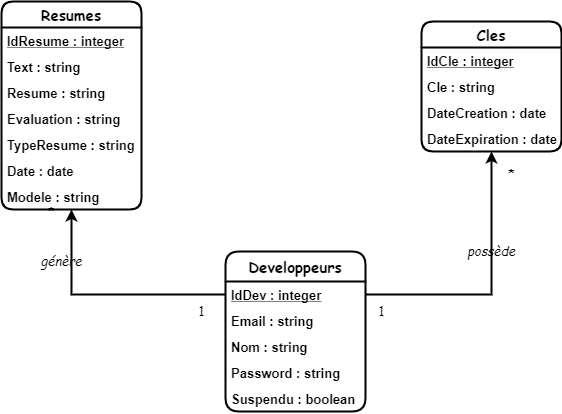
\includegraphics[width=14cm]{BDdiagrams.png}
\captionof{figure}[Structure de la base des données]{Diagramme des classes représentant la base des données} \label{BDdiagrams}
\end{center}
$ _{ } $\\
On peut remarquer sur la figure \ref{BDdiagrams} l'ajout des attributs \underline{type de résumé} et \underline{date} dans la classe des résumés, ainsi que des attributs \underline{date de création} et \underline{date d'expiration} dans la classe des clés d'authentification, puis finalement l'attribut \underline{suspendu?} dans la classe des développeurs.

\begin{itemize}
\item[•] L'attribut \textit{type de résumé} permettra de sélectionner les résumés par type sans avoir à se fier des modèles mis en place dans le système;
\item[•] L'attribut \textit{date} ajouté dans la classe des résumés pourra permettre de suivre l'évolution des performances car on aura également le modèle qui aura produit les résumés considérés.
\item[•] Les attributs \textit{date de création} et \textit{date d'expiration} ajoutés à la classe des clés permettront de faciliter plus tard le management des développeurs utilisateurs des services de l'API dans leurs systèmes et cela va en connivence avec l'attribut \textit{suspendu?} ajouté à la classe des développeurs.
\end{itemize}
Les \textit{id} seront considérés comme clé primaire et l'\underline{id de développeur} sera une clé étrangère dans les tables réservées aux résumés et aux clés. Ainsi, nous considérons terminée la phase de conception de la base des données.
\subsection{Conception de l'API de synthèse}
$ _{} $ $ _{} $ $ _{} $ $ _{} $ $ _{} $La création d'une interface de programmation des applications (\textit{Application Programming Interface}) se fait en s'interrogeant sur les services qu'on veut pourvoir à travers cette \textit{API}.\\
Pour ce qui nous concerne, nous voulons mettre au point une plateforme capable de retourner les résumés aux textes qui lui seront présentés. Nous devons également pouvoir identifier les gens qui se serviront de l'API dans leurs systèmes (les développeurs dont on parlait dans la section précédente), d'où la nécessité de les enregistrer, de leur donner la possibilité de s'authentifier et de générer une clé d'authentification à utiliser dans leurs systèmes.\\
$ _{} $ $ _{} $ $ _{} $ $ _{} $ $ _{} $Nous allons également donner la possibilité de tester plusieurs modèles de résumé des textes et permettre ainsi aux utilisateurs de comparer diverses synthèses. Pour cela, nous avons prévu $ 4 $ familles d'\textit{end-points} :
\begin{itemize}
\item[1°)] \textit{End-points} réservés à la synthèse extractive;
\item[2°)] \textit{End-points} réservés à la synthèse abstractive;
\item[3°)] \textit{End-points} réservés à tout ce qui concerne les vues de l'API (ses interfaces devant permettre l'authentification, la génération des clés et la documentation);
\item[4°)] \textit{End-points} réservés à l'administration du système (que nous avons implémenté mais que nous passerons sous silence dans ce travail).
\end{itemize}
On peut aussi y joindre un \textit{end-poind pour l'évaluation} des résumés produits.
\subsubsection{End-points pour la synthèse extractive}
$ _{} $ $ _{} $ $ _{} $ $ _{} $ $ _{} $Pour la synthèse extractive, nous avons prévu essentiellement deux \textit{end-points} pour comparer notre algorithme de synthèse extractive à l'un des systèmes de synthèse extractive le plus performant. Il s'est agit des \textit{end-points} réservé au système basé sur le module python \textit{gensim} et celui réservé à notre approche qui est un mélange de plusieurs algorithmes de synthèse extractive (on l'a nommé \textit{merging}) comme on peut le voir sur la figure \ref{ArchiGlobExtract} du chapitre précédent.\\
On a l'\textit{end-point} de synthèse extractive basé sur le module \textit{gensim} donné par :
\begin{center}

\includegraphics[scale=0.5]{POSTextractiveGensim.png}
\end{center}
Puis celui de synthèse extractive par combinaison de divers algorithmes donné par :
\begin{center}

\includegraphics[scale=0.5]{POSTextractiveMerge.png}
\end{center}
\subsubsection{End-points pour la synthèse abstractive}
Pour la synthèse abstractive, nous avons prévu $ 5 $ \textit{end-points} dont :
\begin{itemize}
\item[1.] Un \textit{end-point} utilisant le modèle \textit{BART} dont nous avons optimisé l'utilisation en le servant à travers le processus présenté à la figure \ref{PipelineSumm} du chapitre précédent. L'\textit{end-point} en question est :
\begin{center}

\includegraphics[scale=0.5]{POSTabstractiveLarge.png}
\end{center}
\item[2.] Un autre \textit{end-point} basé sur \textit{BART} mais pouvant prendre en charge des documents plus gros :
\begin{center}

\includegraphics[scale=0.5]{POSTabstractiveVeryLarge.png}
\end{center}
\item[3.] Un \textit{end-point} basé sur \textit{BARThez}, le modèle de synthèse le plus utilisé pour la synthèse entièrement en français :
\begin{center}

\includegraphics[scale=0.5]{POSTabstractiveBarthez.png}
\end{center}
\item[4.] Un \textit{end-point} basé sur \textit{Pegasus}, l'un des modèles à grand pouvoir d'abstraction :
\begin{center}

\includegraphics[scale=0.5]{POSTabstractivePegasus.png}
\end{center}
\item[5.] Un \textit{end-point} basé sur \textit{BARTkrame}, notre modèle de synthèse élaboré pour fonctionner entièrement en français :
\begin{center}

\includegraphics[scale=0.5]{POSTabstractiveExperimentalBartkrame.png}
\end{center}
\end{itemize}
\subsubsection{End-points pour les vues de l'API et l'authentification}
Tout d'abord, le point d'entrée est donné naturellement par l'\textit{end-point} :
\begin{center}

\includegraphics[scale=0.5]{GEThome.png}
\end{center}
Ensuite, l'\textit{end-point} réservé à l'authentification :
\begin{center}

\includegraphics[scale=0.5]{POSTlogin.png}
\end{center}
Vient alors l'\textit{end-point} dédié à l'enregistrement :
\begin{center}

\includegraphics[scale=0.5]{POSTsignUp.png}
\end{center}
Par après on a l'\textit{end-point} réservé à la déconnexion :
\begin{center}

\includegraphics[scale=0.5]{GETlogout.png}
\end{center}
Puis celui réservé à la génération des clés :
\begin{center}

\includegraphics[scale=0.5]{GETupdateToken.png}
\end{center}

Finalement, on a un \textit{end-point} commun aux familles de synthèse extractive et abstractive pour l'évaluation des synthèses. C'est donné par :
\begin{center}

\includegraphics[scale=0.5]{POSTevaluation.png}
\end{center}
$ _{ } $\\
Nous estimons que la description ici faite suffit comme conception des grandes lignes de notre \textit{API}. Le reste de la documentation est dans l'annexe \ref{AnnexeDocu}.
\subsection{Conception des interfaces}\label{SectionConceptionInterfaces}
$ _{} $ $ _{} $ $ _{} $ $ _{} $ $ _{} $Étant donné l'API mise sur pieds, nous avons également implémenté un client web devant s'en servir pour en illustrer le fonctionnement. Pour cela, nous avons voulu exploiter toutes les possibilités de l'API en se basant sur les spécifications du système (nous les avons cité au chapitre précédent) et les objectifs de ce travail. C'est ainsi que les interfaces ont été conçues de manière à pouvoir :
\begin{itemize}
\item[•] Permettre la synthèse abstractive en utilisant tous les modèles mis à notre disposition par l'API;
\item[•] Permettre la synthèse extractive en utilisant les deux approches pourvues par l'API;
\item[•] Permettre le téléchargement des synthèses obtenues;
\item[•] Permettre aux utilisateurs de coter les synthèses qui leur ont été fournies;
\item[•] Permettre le chargement des fichiers sous différents formats (\textbf{word}, \textbf{pdf} et \textbf{txt}).
\end{itemize}
Pour cela, et sur base de l'ébauche des interfaces qui a été présentée à la figure \ref{EbaucheInterface} nous avons adopté ce qui suit comme interfaces du client de notre système.
\begin{center}
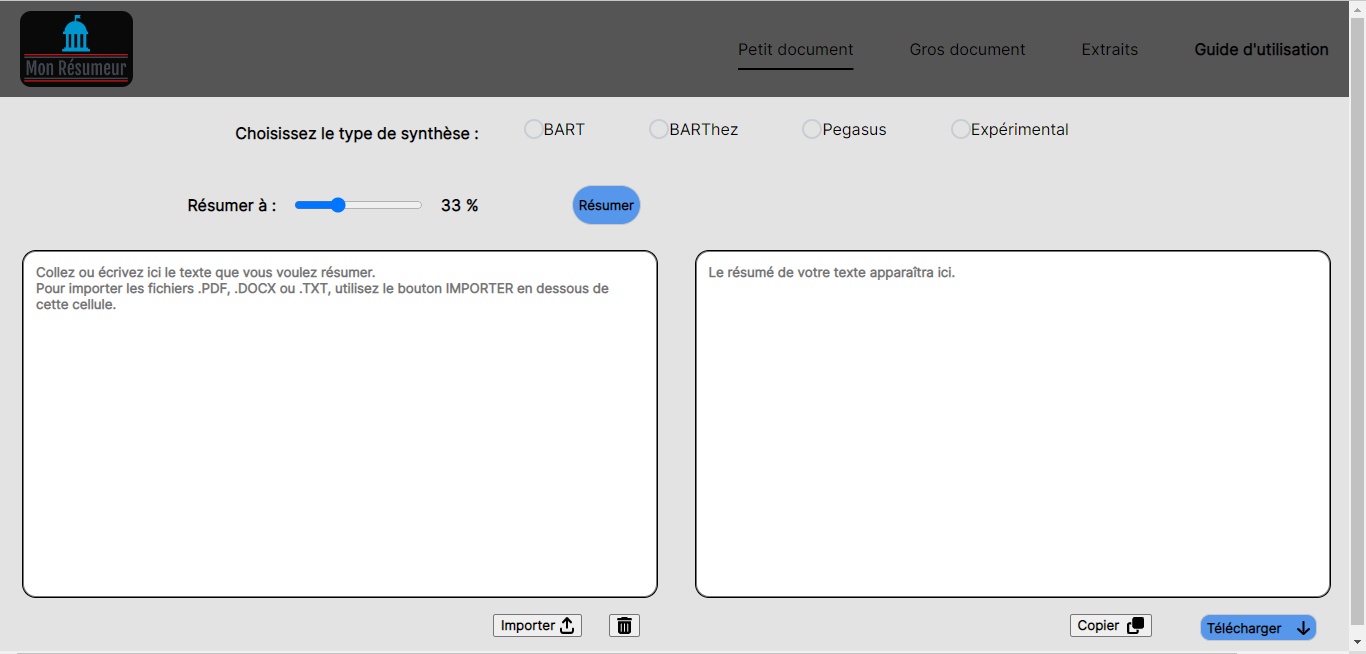
\includegraphics[width=16cm]{Interface1PetitsDocs.png}
\captionof{figure}{Interface générique du système}\label{Interface1PetitsDocs}
\end{center}
Sur la figure \ref{Interface1PetitsDocs} nous montrons la manière dont les interfaces se présentent en général.\\
Durant le processus de synthèse, l'interface se présente comme suit :
\begin{center}
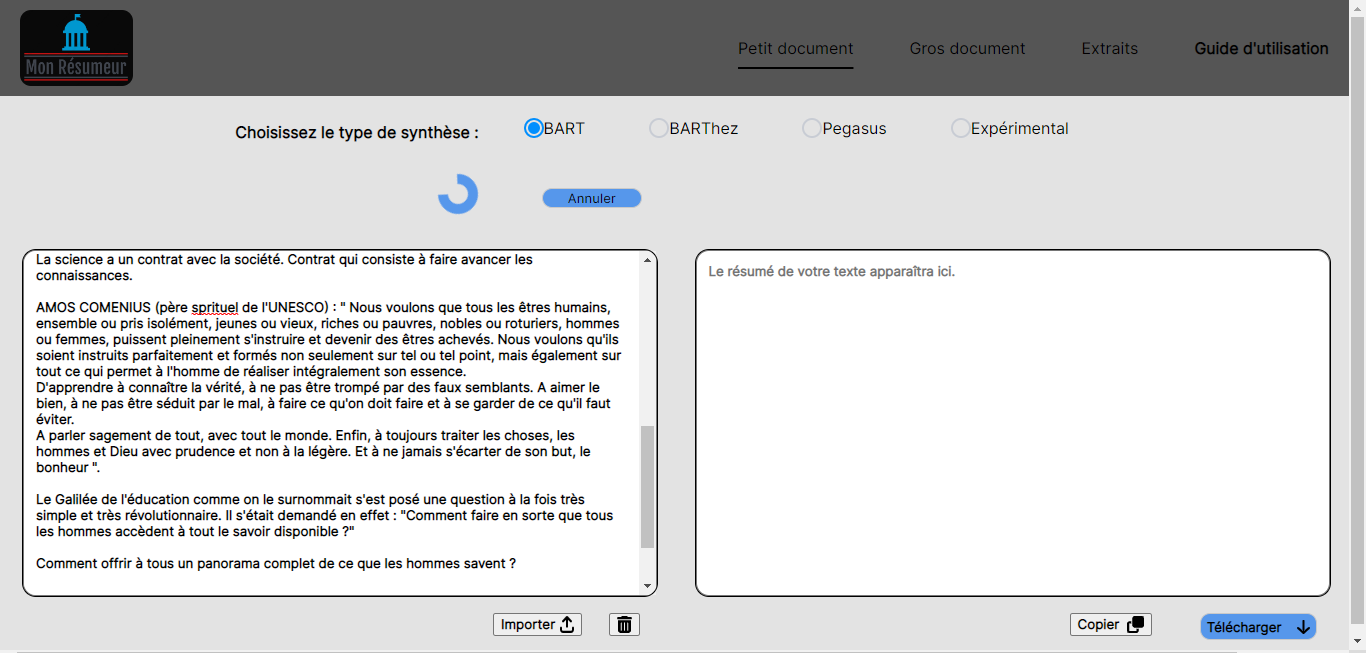
\includegraphics[width=16cm]{Interface1Pendant.png}
\captionof{figure}{Interface durant le processus de synthèse}\label{Interface1EnCours}
\end{center}
On peut remarquer sur la figure \ref{Interface1EnCours} que durant la synthèse, une possibilité d'annulation se présentera.\\
Après génération de la synthèse, l'interface se présentera comme suit :
\begin{center}
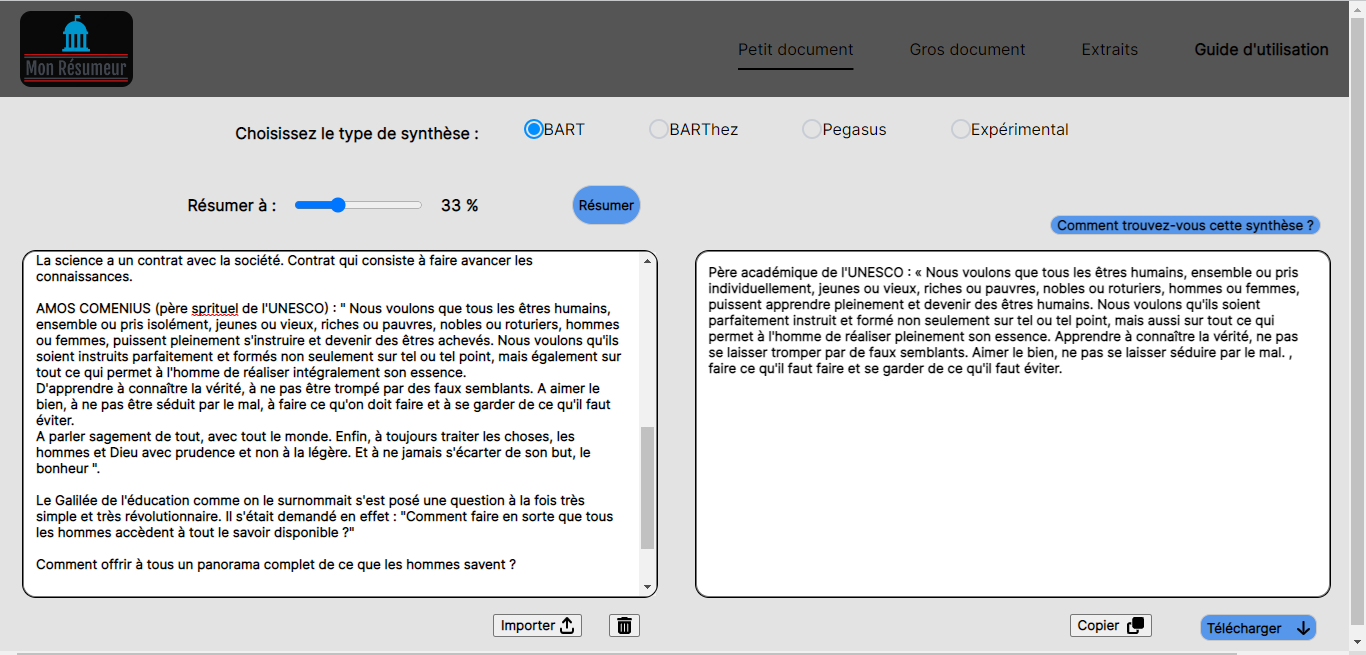
\includegraphics[width=16cm]{Interface1Apres.png}
\captionof{figure}{Interface après génération de la synthèse}\label{Interface1Apres}
\end{center}
Il est clair également sur la figure \ref{Interface1Apres} qu'après synthèse, un bouton devant permettre d'évaluer la synthèse se présentera. En y cliquant, on pourra avoir la possibilité d'évaluer le résumé obtenu, comme cela se voit sur la figure suivante :
\begin{center}
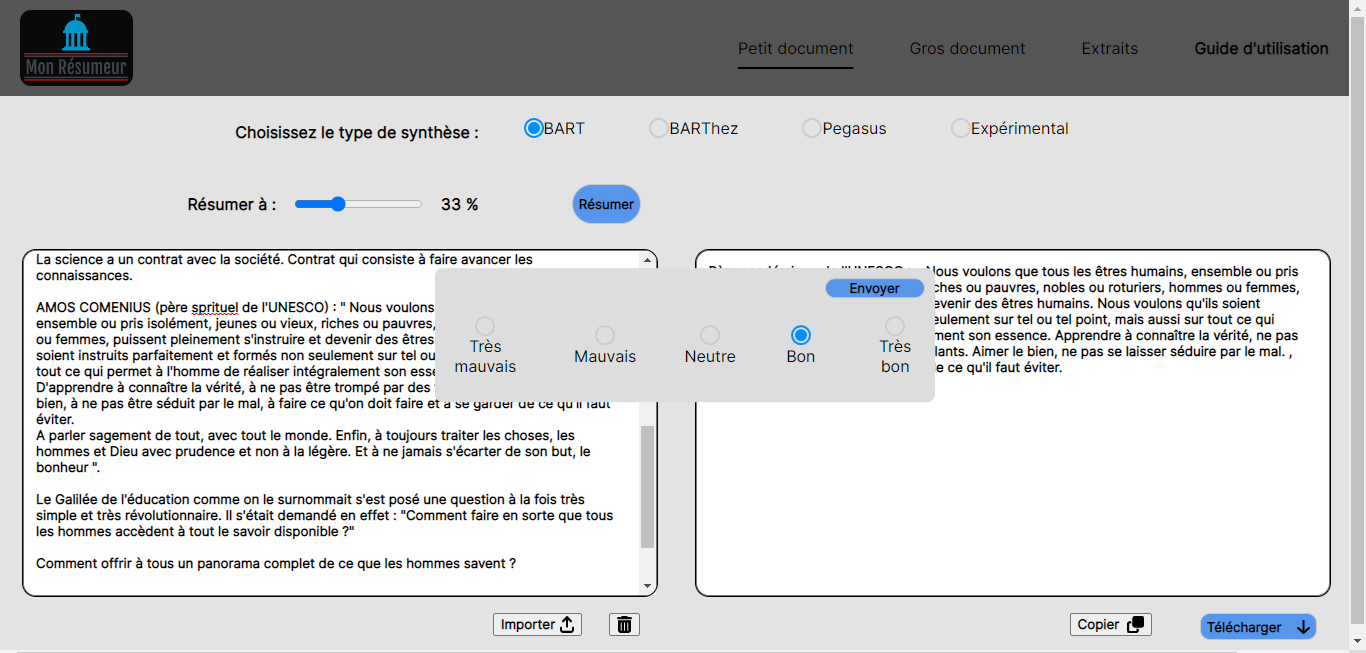
\includegraphics[width=16cm]{Interface1Evaluation.png}
\captionof{figure}{Interface durant l'évaluation de la synthèse obtenue}\label{Interface1Evaluation}
\end{center}
Pour guider l'utilisateur, au survol du curseur de réglage de la taille du résumé, l'interface se présente comme suit :
\begin{center}
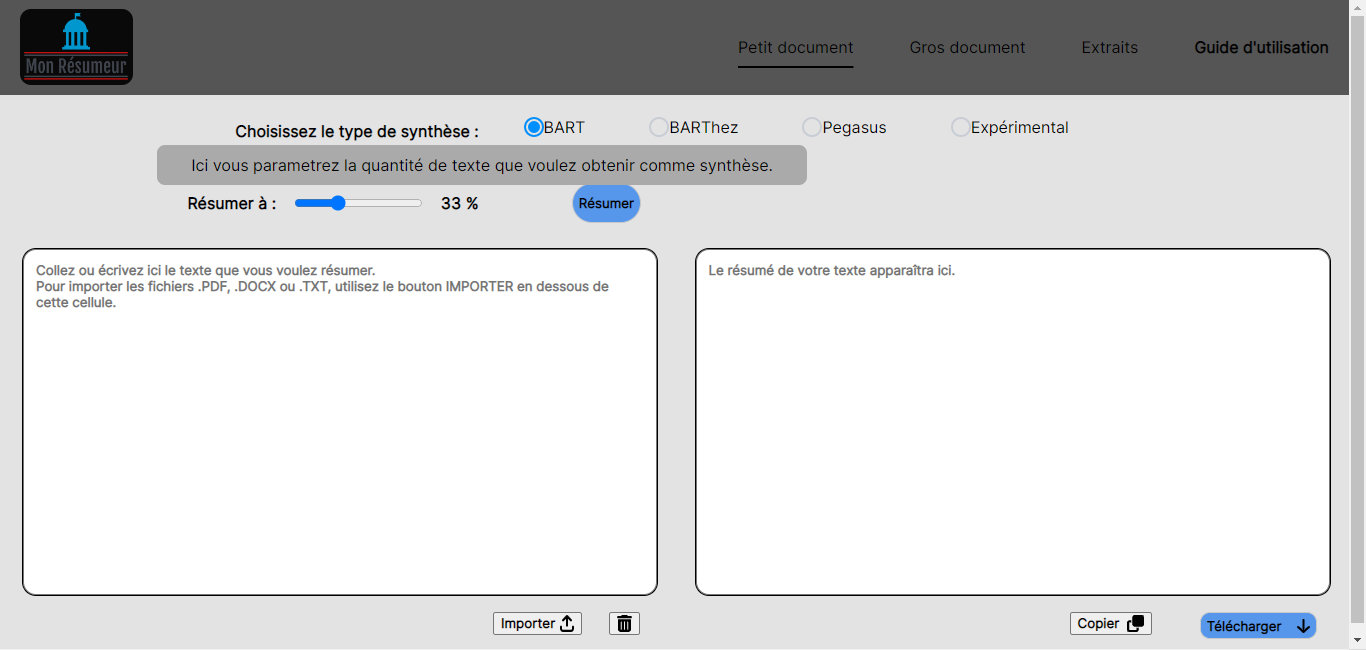
\includegraphics[width=16cm]{Interface1CurseurHover.png}
\captionof{figure}{Interface au survol du curseur de réglage de résumé}\label{Interface1CurseurHover}
\end{center}

En cas de limitation des ressources serveur lors de l'hébergement de l'API, nous avons prévu disponibiliser uniquement le système réduit :
\begin{center}
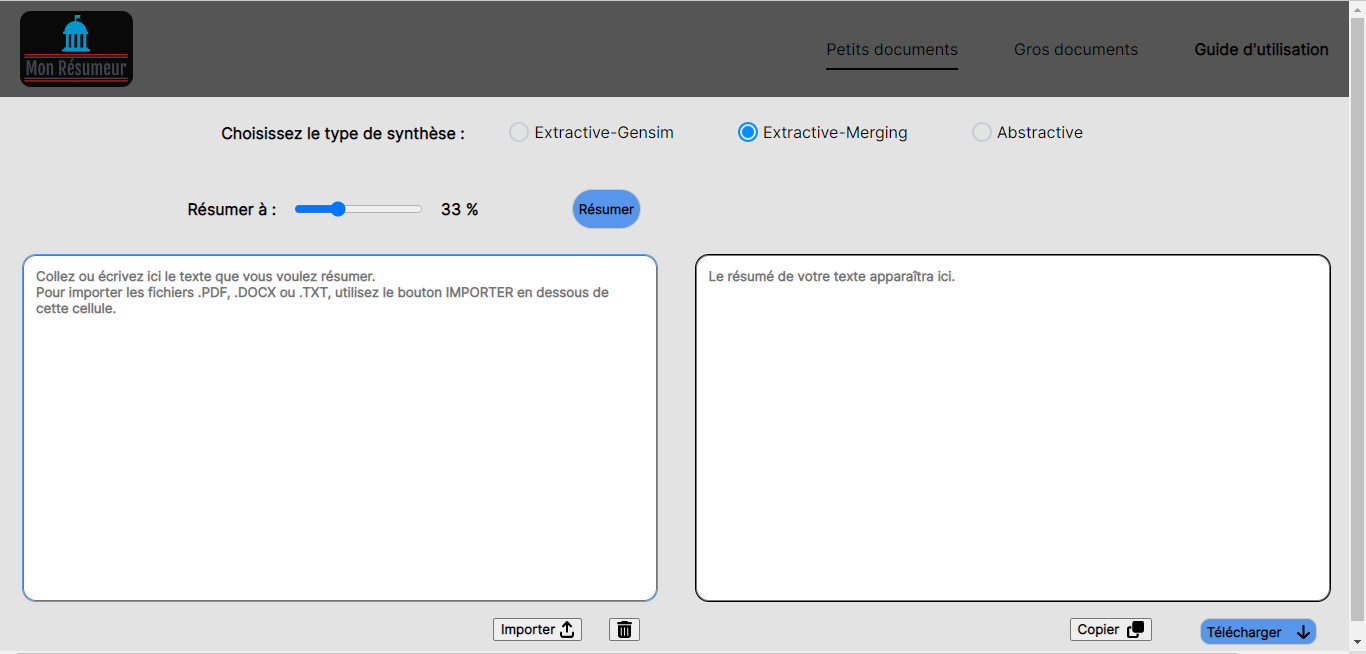
\includegraphics[width=16cm]{InterfacesReducedPetitsDocs.png}
\captionof{figure}{Interface réduite côté petits documents}\label{InterfacesReducedPetitsDocs}
\end{center}

\begin{center}
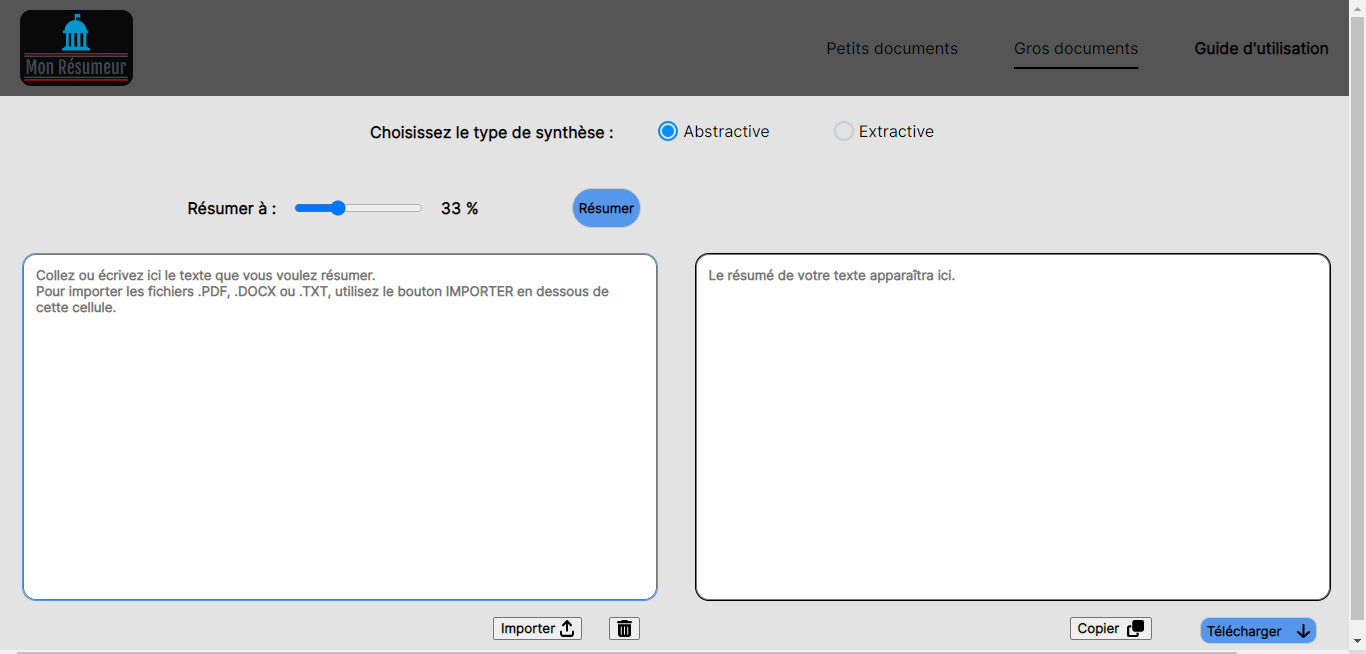
\includegraphics[width=16cm]{InterfacesReducedGrosDocs.png}
\captionof{figure}{Interface réduite côté gros documents}\label{InterfacesReducedGrosDocs}
\end{center}

Les autres fonctionnalités peuvent être explorées en utilisant le système.

\section{Évaluation des résumés}\label{sectionSurROUGE}
$ _{} $ $ _{} $ $ _{} $ $ _{} $ $ _{} $L'évaluation des résumés est une tâche assez complexe. Les méthodes cla\-ssi\-que\-ment utilisées pour évaluer les performances d'un système informatique, et en particulier celles utilisées pour évaluer les systèmes basés sur les réseaux de neurones, ne peuvent pas s'appliquer de manière brute pour les systèmes de génération de texte comme ceux de résumé automatique. En effet, il n'existe pas de référence parfaite de résumé pour un document donné. Les professionnels humains d'ailleurs produisent des résumés différents pour un même texte, chacun selon ses penchants et ses goûts. Plus étonnant encore, un même humain ne produit en général pas le même résumé si la tâche lui est donnée à quelques temps d'intervalle \cite{rath1961formation}. C'est donc une tâche teintée d'une grande part de subjectivité. Cependant, la majorité s'accorde quand on est face à un bon résumé.\\
$ _{} $ $ _{} $ $ _{} $ $ _{} $ $ _{} $Comment alors faire pour parvenir à repérer, avec plus d'objectivité, qu'un résumé donné est de bonne qualité ? Comment même parvenir à comparer, sans équivoque, les qualités de deux résumés qui nous seraient présentés ? La solution à cette question est importante car elle permettra de pouvoir évaluer objectivement et rapidement les systèmes de résumé automatique mais, au-delà de cela, elle permettra d'en suivre l'évolution durant l'entraînement au cas où il s'agit des systèmes de résumé basés sur l'apprentissage automatique.\\
$ _{} $ $ _{} $ $ _{} $ $ _{} $ $ _{} $Généralement, on subdivise l'évaluation des résumés en deux principales catégories qui sont l'évaluation extrinsèque et l'évaluation intrinsèque\cite{jones1995evaluating}. L'évaluation intrinsèque est celle qui s'obtient par la lecture directe du résumé. Il peut s'agir d'un résumé manuel (évaluation directe par un humain selon un certain nombre de critères), un résumé semi-automatique ou bien un résumé automatique. L'évaluation extrinsèque quant à elle consiste à évaluer les résumés indirectement. Pour ce faire, on peut par exemple passer par l'évaluation de la possibilité de donner une réponse à un certain nombre de questions après lecture du résumé \cite{maybury1999advances},... Beaucoup de recherches ont été menées sur l'évaluation des résumés mais les solutions ne sont que partielles le plus souvent \cite{lin2004rouge,hirschberg2005summaries,louis2008automatic, saggion2010multilingual}. Dans ce travail, nous ne parlons que des méthodes d'évaluation intrinsèques qui nous intéressent.
\subsection{Évaluation manuelle}
$ _{} $ $ _{} $ $ _{} $ $ _{} $ $ _{} $L'évaluation manuelle consiste à se fier au jugement d'un certain nombre d'experts humains, selon un certain nombre de critères préétablis \cite{torres2014automatic}. Pour plus d'information à ce sujet, se rapporter aux campagnes annuelles d'évaluation \textbf{DUC} ou \textit{Document Understanding Conference} (renommé \textbf{TAC} \cite{TAC} ou \textit{Text Analysis Conference} depuis $ 2008 $). Ces méthodes demeurant subjectives, les méthodes semi-automatiques ont été mises au point.
\subsection{Évaluation semi-automatique}
$ _{} $ $ _{} $ $ _{} $ $ _{} $ $ _{} $Nous allons présenter ici les méthodes les plus connues et les plus utilisées \cite{hong2014repository} pour évaluer les résumés. Il s'agit de \textbf{ROUGE}(\textit{Recall Oriented Understudy for Gisting Evaluation}), \textit{que nous allons utiliser pour nos évaluations} et de \textbf{PYRAMID} dont nous allons montrer la faiblesse par rapport à \textit{ROUGE}, bien que celui-là soit plus corrélé aux jugements humains \cite{nenkova2004evaluating}.
\subsubsection{ROUGE \cite{lin2004rouge}}\label{ROUGEmetricsSection}
$ _{} $ $ _{} $ $ _{} $ $ _{} $ $ _{} $Cette métrique est orientée rappel comme son nom l'indique. On cherche à évaluer jusqu'à quel point le résumé obtenu rappelle celui qui est pris comme référence. Pour réaliser ladite mesure, on se base essentiellement sur la correspondance mot à mot (on parle des \textit{unigrammes}), de deux mots à deux mots (on parle alors de comparaison par \textit{bigrammes}),... Pour être général, on parle des \textit{n-grammes}. Considérons la phrase :
\begin{center}
\textit{Il arrive demain avec deux objets rares.}
\end{center}
Les unigrammes de cette phrase sont \textit{il}, \textit{arrive}, \textit{demain}, \textit{avec}, \textit{deux}, \textit{objets} et \textit{rares}, soit les mots du texte. Les bigrammes sont \textit{il arrive}, \textit{arrive demain}, \textit{demain avec}, \textit{avec deux}, \textit{deux objets}, \textit{objets rares}.
Dans le paquet des mesures proposées par \textit{ROUGE}, il y a :
\begin{itemize}
\item[1°)] \underline{ROUGE-N}\\
Formellement, \textit{ROUGE-N} est une mesure de rappel (\textit{recall}) des N-grammes entre le résumé candidat et le ou les résumé(s) de référence. C'est régi par la relation qui suit :
\begin{eqnarray}
ROUGE-N = \frac{\sum_{r\in R}\mbox{ }Co_{c-r}}{\sum_{r\in R}\mbox{ }(N-grammes)_{r}}
\end{eqnarray}
Avec $ r $ un résumé de référence parmi ceux pris pour référence (paquet $ R $), $ (N-grammes)_{r} $ le nombre total de \textit{N-grammes} dans un résumé de référence \textit{r} et $ Co_{c-r} $ le nombre de \textit{N-grammes} du résumé candidat qui se retrouvent dans le résumé de référence \textit{r}.\\
C'est ainsi qu'on trouve \textit{ROUGE-1} basé sur une comparaison des \textit{unigrammes}, \textit{ROUGE-2} basé sur celle des \textit{bigrammes},... \textit{ROUGE-2} est particulièrement jugée très efficace pour l'évaluation des résumés\cite{MaaliMnasri}.
\item[2°)] \underline{ROUGE-L}\\
Il s'agit cette fois d'une mesure \textit{ROUGE} basée non pas sur des n-grammes comme tel, mais plutôt sur l'évaluation des plus longues sous-séquences communes entre les phrases du résumé candidat avec celles du résumé de référence. Pour faire simple, considérons un résumé candidat $ X $ et un résumé de référence $ Y $. Si $ m $ est le nombre d'unigrammes contenus dans $ X $ et $ m $ celui de $ Y $ on va définir deux rappels (sur $ X $ et sur $ Y $) donnés par :
\begin{eqnarray}
R_{X} = \frac{LCS(X,Y)}{m} \label{EqROUGE_L1}\\
R_{Y} = \frac{LCS(X,Y)}{n} \label{EqROUGE_L2}
\end{eqnarray}
Les expressions \ref{EqROUGE_L1} et \ref{EqROUGE_L2} nous permettent finalement de définir la mesure \textit{ROUGE-L} par :
\begin{eqnarray}
ROUGE-L = \frac{(1+\beta^{2}) R_{X}R_{Y}}{R_{X}+\beta^{2}R_{Y}}\label{EqROUGE_L}
\end{eqnarray}
Dans les expressions \ref{EqROUGE_L1}, \ref{EqROUGE_L2} et \ref{EqROUGE_L}, $ LCS(X,Y) $ désigne la plus longue séquence commune à $ X $ et $ Y $. On la nomme habituellement \textit{Long Common Subsequence} (\textit{\textbf{LCS}}). Pour illustration, considérons deux phrases :
\begin{center}
$ A =  $ \textit{\underline{Nous} voulons \underline{savoir ce qui se} passera.}\\
$ B =  $ \textit{\underline{Nous} finirons par \underline{savoir ce qui se} passe.}
\end{center}
On remarque que la plus longue sous-séquence commune à $ A $ et $ B $ est \textit{nous savoir ce qui se}, donc $ LCS(A,B) = 5 $. Il faut noter qu'ici nous n'avons décrit que la procédure de calcul de \textit{ROUGE-L} pour des résumés à une phrase. Néanmoins, pour un résumé à plusieurs phrases, l'idée est la même mais la comparaison est faite phrase après phrase \cite{lin2004rouge}.
\item[3°)] \underline{ROUGE-S}\\
Cette méthode se base sur ce qu'on nomme les \textit{skip-bigrammes} pour évaluer les résumés. Cela correspond à utiliser les bigrammes sans se limiter au fait que les termes soient consécutifs. Par exemple, dans la phrase : 
\begin{center}
\textit{La terre semble être plate}
\end{center}
On a les \textit{skip-bigrammes} suivants : \textit{la terre}, \textit{la semble}, \textit{la être}, \textit{la plate}, \textit{terre semble}, \textit{terre être}, \textit{terre plate}, \textit{semble être}, \textit{semble plate} et finalement \textit{être plate}, soit $ 10 $ \textit{skip-bigrammes}. On a en fait toujours $ C_{n}^{2} $ \textit{skip-bigrammes} avec $ n $ le nombre d'unigrammes dans la phrase considérée. Pour notre cas, il s'agit de $ 5 $ unigrammes et on a bel et bien $ C_{5}^{2}=\frac{5!}{3!2!} = 10 $. Après cela, on établit des relations du même type que celles établies pour \textit{ROUGE-L} (voir la relation  \ref{EqROUGE_L}).
\end{itemize}
Il faut noter que des améliorations peuvent être apportées à ces méthodes pour avoir d'autres variantes. Cela permet d'obtenir \textit{ROUGE-S} avec un \textit{gap maximal} (séparation maximale entre \textit{N-grammes} formant les \textit{skip-bigrammes}), \textit{ROUGE-SU}\textit{ROUGE-LSum} et\\ \textit{ROUGE-W} par exemple. Pour plus de détails à ce sujet, on peut regarder l'article fondateur du paquet d'évaluation \textit{ROUGE} \cite{lin2004rouge}.\\
Il faudra noter également que l'une des sources du succès de \textit{ROUGE} est sa facilité d'im\-plé\-men\-ta\-tion une fois qu'on a déjà des résumés de référence, ainsi que sa grande corrélation avec les jugements humains \cite{lin2004rouge,MaaliMnasri, hong2014repository}.
\subsubsection{PYRAMID \cite{nenkova2004evaluating}}
$ _{} $ $ _{} $ $ _{} $ $ _{} $ $ _{} $Cette méthode permet de comparer un résumé candidat à un ensemble de résumés de référence. L'inconvénient de cette méthode est que, par essence, elle exige l'existence de plusieurs résumés de référence, ce qui n'est pas exigé pour la méthode \textit{ROUGE}.\\
$ _{} $ $ _{} $ $ _{} $ $ _{} $ $ _{} $\\
$ _{} $ $ _{} $ $ _{} $ $ _{} $ $ _{} $Les méthodes semi-automatiques peuvent être vues comme automatique au cas où trouver les résumés de référence ne pose aucun problème. Malheureusement, cela ne suffit pas car la subjectivité est considérée comme étant aussi un facteur de biais. D'où l'émergence des méthodes  automatiques.
\subsection{Évaluation automatique}
$ _{} $ $ _{} $ $ _{} $ $ _{} $ $ _{} $Les méthodes d'évaluation automatiques réalisent l'évaluation en se basant uniquement sur le résumé obtenu et le texte résumé (texte d'origine). La non exigibilité des références rend ces méthodes particulièrement intéressantes.\\
Nous n'avons pas utilisé ces méthodes d'évaluation dans ce travail, en plus, elles ne sont pas encore mûres \cite{MaaliMnasri,louis2008automatic,radev2003evaluation}.
\section{Description succincte de l'implémentation}
$ _{} $ $ _{} $ $ _{} $ $ _{} $ $ _{} $Comme on peut le voir sur la figure \ref{ArchiSysteme}, notre système est conçu selon l'architecture trois tiers. Nous avons donc la partie cliente et la partie serveur. Néanmoins, s'agissant de notre système (que nous avons dénommé \textit{Mon Résumeur}), cette distinction n'est pas trop claire. Nous allons donc préciser clairement les éléments qui le constituent. L'im\-plé\-men\-ta\-tion du système a été faite en considérant les parties suivantes :
\begin{itemize}
\item[1°)] Une \textit{API REST} que nous avons implémenté pour le traitement des données lui envoyés par les parties clientes. Le traitement en question consiste à synthétiser le texte qui lui est fourni, d'envoyer le résultat de ce traitement au système demandeur et de stocker les résultats du processus. Cette \textit{API}, tel que nous l'avons implémenté est constituée d'une partie \textit{frontend} et d'une partie \textit{backend}. Le \textit{frontend} c'est pour permettre aux programmeurs de se documenter sur les \textit{end-points} disponibilisés par l'\textit{API} et leur fonctionnement, tout en leur permettant de s'authentifier pour pouvoir utiliser les services de l'\textit{API} dans leurs systèmes respectifs.
\item[2°)] Du point 1° on comprend directement qu'il y a également une base des données. Pour cette première version de notre système, nous avons d'abord opté pour une base de données du type \textit{SQLite}.
\item[3°)] Une partie cliente qui a également un \textit{frontend} et un \textit{backend}. Cette partie a été implémentée pour montrer que l'\textit{API} que nous avons mis au point est bel et bien utilisable. N'importe quel autre programmeur ayant les autorisations nécessaires peut donc se servir de l'API dans son système. Pour notre cas, le système que nous avons mis au point pour utiliser l'\textit{API} a une partie \textit{frontend} devant permettre aux utilisateurs de charger leurs documents et une partie \textit{backend} devant permettre de réaliser quelques traitements avant d'envoyer les documents chargés par les u\-ti\-li\-sa\-teurs. Ce petit traitement du début à pour objectif de corriger les erreurs de présentation de textes qui peuvent subvenir selon les outils et les langages utilisés pour cette fin.
\end{itemize}
\subsection{API REST}
\subsubsection{Partie \textit{frontend}}
$ _{} $ $ _{} $ $ _{} $ $ _{} $ $ _{} $Quelques captures de la partie \textit{frontend} de l'\textit{API} sont mises à l'annexe \ref{AnnexeFrontAPI}. Cette partie a été faite en utilisant \textit{HTML}, \textit{CSS} et très peu de \textit{JavaScript} pour la génération des clés par les programmeurs voulant utiliser l'\textit{API}. Ce \textit{frontend} permet donc aux programmeurs de s'authentifier et de générer leurs clés mais également de consulter la documentation de l'\textit{API}. 
\subsubsection{Partie \textit{backend}}
$ _{} $ $ _{} $ $ _{} $ $ _{} $ $ _{} $Cette partie est le coeur du système. C'est dans elle que nous implémentons les divers algorithmes de synthèse ainsi que la gestion des requêtes des utilisateurs. Elle a été réalisée en utilisant le \textit{framework Python} dénommé \textit{\textbf{Flask}} vu que nous avons implémenté nos algorithmes de synthèse en Python. Cette partie disponibilise plusieurs \textit{end-points} comme on peut le voir dans la documentation mise à l'annexe \ref{AnnexeDocu}.\\
Les précisions sur l'implémentation des algorithmes de cette partie sont les suivantes :
\begin{itemize}
\item[•] Pour la \textit{synthèse extractive simplifiée} nous avons utilisé le module python dénommé \textit{\textbf{Gensim}}.
\item[•] Pour la synthèse que nous avons réalisé en mélangeant divers algorithmes, nous avons modifié le module python \textit{\textbf{sumy}} (version $ 0.0.1 $). Nous l'avons modifié de manière à pouvoir accéder aux poids et non aux synthèses, de manière à pouvoir mieux contrôler le ratio, de manière à y ajouter l'algorithme \textit{Tf-Idf} et à le rendre compatible à la langue française. Cela avec aussi comme objectif d'avoir un contrôle total sur le pré-traitement, de l'uniformiser pour tous les algorithmes (même \textit{tokenizer} pour tous) et de combiner les sorties selon l'algorithme conçu à la section \ref{SectionMerging}.
\item[•] Pour la synthèse des petits documents, nous avons utilisé le \textit{transformer} \textit{BART} que nous avons servi à travers le pipeline décrit à la figure \ref{PipelineSumm}, en ajustant également les longueurs des entrées aux tailles que nous avons jugé optimales pour réduire la complexité de calcul, car les modèles du type \textit{transformer} ont une \textit{complexité algorithmique linéaire en la longueur de leurs têtes d'attention mais quadratique en la longueur des séquences d'entrée} \cite{vaswani2017attention}. Dans cette partie dédiée aux petits documents, nous avons également ajouté le \textit{transformer} \textit{BARThez} ainsi que notre \textit{transformer} basé sur \textit{mBART} et que nous serons entrain d'améliorer au fil de l'utilisation du système. Nous avons mis \textit{BARThez} juste pour avoir un point de repère (de comparaison) en français.\\
Le modèle \textit{BART} étant en anglais, nous devons préciser que notre \textit{API} passe par l'API de \textit{google translate} pour pouvoir tout présenter en français. Notre modèle dit \textit{expérimental} ainsi que \textit{BARThez} n'ont pas eu besoin de traduction car ils sont complètement en français. 
\item[•] Pour la partie \textit{gros documents}, pour la synthèse abstractive, nous avons juste appliqué le modèle \textit{BART optimisé} tel que nous venons de le décrire de manière à pouvoir prendre en compte des documents plus longs sans perte de qualité. Pour cela, la partie a juste consisté à appliquer notre pipeline d'optimisation (figure \ref{PipelineSumm}) au complet. Pour la synthèse extractive des longs documents, nous avons utilisé \textit{gensim} à cause de sa rapidité.
\end{itemize}
Concernant des précisions supplémentaires sur nos modèles et les résultats, il faudra se rapporter à la section \ref{sectioTestEtResultats}.
\subsection{Système client}
$ _{} $ $ _{} $ $ _{} $ $ _{} $ $ _{} $Le système client que nous avons implémenté est également constitué de deux parties principales dont le \textit{backend} et le \textit{frontend}.\\
Le \textit{frontend} correspond à ce que nous avons présenté quand nous avons traité de la con\-ce\-ption des interfaces dans ce travail (il s'agit du point \ref{SectionConceptionInterfaces}). La partie visible (\textit{frontend}) a été réalisée en utilisant le \textit{framework} \textit{JavaScript} dénommé \textit{ReactJS}.\\
Le \textit{backend} pour cette partie, nous a juste permis de réaliser l'extraction des textes et le formatage avant envoi à l'\textit{API}. Il a été réalisé en se servant du module \textit{NodeJS} dénommé \textit{ExpressJS}. Pour cette partie, nous n'avons prévu ni authentification, ni stockage mais cela peut évidemment être fait selon le choix du programmeur se servant de l'\textit{API} de synthèse dans son système.

\section{Tests et interprétation des résultats}\label{sectioTestEtResultats}
$ _{} $ $ _{} $ $ _{} $ $ _{} $ $ _{} $Dans cette partie, chaque fois que nous parlerons de \textit{checkpoint} ou de \textit{point d'entrée}, il faudra comprendre qu'il s'agit du nom du modèle ou bien du \textit{dataset} sur la plateforme \textit{Hugging Face}\footnote{\href{https://huggingface.co}{https://huggingface.co}}. Nous devons également souligner que les résultats \textit{ROUGE} sont ici présentés en pourcentage et plus c'est élevé, plus le modèle considéré peut être quan\-ti\-ta\-ti\-ve\-ment jugé performant sur le \textit{dataset} pris comme référence (pour plus de précisions sur le paquet \textit{ROUGE}, voir la section \ref{ROUGEmetricsSection}).
\subsection{\textit{Datasets} utilisés pour les tests}
$ _{} $ $ _{} $ $ _{} $ $ _{} $ $ _{} $En parlant des tests, nous voulons dire ceux réalisés pour évaluer les performances des modèles les uns par rapport aux autres. Pour cela, il nous est nécessaire d'utiliser les mêmes \textit{datasets} ainsi que les mêmes métriques de mesure des performances. Les \textit{datasets} que nous avons utilisés font partie de ceux qui sont généralement utilisés dans divers \textit{benchmarks} dédiés à la synthèse automatique.\\
Ainsi, nous avons utilisé les \textit{datasets} \textit{\textbf{CNN / DailyMail}} (version $ 3.0.0 $ ), \textit{\textbf{XSum}}, \textit{\textbf{OrangeSum}} et \textit{\textbf{for-ULPGL-Dissertation}} (Version $ 0.0.1 $, la première version). Tous ces \textit{datasets} sont accessibles sur \textit{Hugging Face}\footnote{\href{https://huggingface.co/datasets/}{https://huggingface.co/datasets/}} et sont constitués de trois sous-catégories dont les données de \textit{test}, les données d'\textit{entraînement}, ainsi que les données de \textit{validation}.
\subsubsection{\textit{Dataset} CCN / DailyMail}
$ _{} $ $ _{} $ $ _{} $ $ _{} $ $ _{} $Le jeu de données \textit{CNN / DailyMail} est un jeu de données en langue anglaise contenant un peu plus de 300 000 articles d'actualité uniques, rédigés par des journalistes des chaînes \textit{CNN} et du \textit{Daily Mail}. La version actuelle prend en charge le résumé extractif et abstractif, bien que la version originale ait été créée pour la lecture et la compréhension automatiques et la réponse aux questions abstractives \footnote{\href{https://huggingface.co/datasets/ccdv/cnn\textunderscore dailymail}{https://huggingface.co/datasets/ccdv/cnn\textunderscore dailymail}}.\\
Pour nos tests, nous avons utilisé la \textbf{version $ 3.0.0 $} retrouvable au point d'entrée\\ \textbf{ccdv/cnn\textunderscore dailymail}. Ce qui veut dire qu'on peut le télécharger en utilisant les lignes de code python suivantes :
\begin{center}
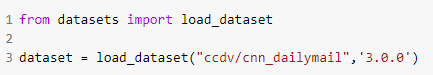
\includegraphics[scale=1]{SnippetCnnDailyMail.png}
\end{center}
Code à utiliser en ayant installé au préalable le module \textit{datasets} grâce à \textit{pip install datasets}.
\subsubsection{\textit{Dataset} XSUM}
$ _{} $ $ _{} $ $ _{} $ $ _{} $ $ _{} $Il s'agit d'un jeu de données de résumés de nouvelles avec des résumés gé\-né\-ra\-le\-ment qualifiés très abstraits. Ces données ont été constituées en collectant des articles en ligne de la \textit{BBC} (\textit{British Broadcasting Corporation}) qui sont accompagnés des petits résumés. Il s'agit d'un jeu de données en anglais donc. Plus précisément, chaque article est précédé d'une phrase d'introduction (appelée résumé) rédigée par un professionnel, généralement l'auteur de l'article. Le résumé porte la classe HTML "storybody introduction" et peut être facilement identifié et extrait du corps du texte principal. Ce \textit{dataset} a été introduit dans l'article \cite{XSumArticle} et tous les détails sur sa formation et ses spécificités peuvent y être trouvés.\\
En ce qui nous concerne, nous avons utilisé la version retrouvable sur \textit{hugging face} au \textit{chekpoint} éponyme \textbf{xsum} \footnote{\href{https://huggingface.co/datasets/xsum}{https://huggingface.co/datasets/xsum}}. Ce qui veut dire qu'il peut être chargé avec \textit{python} grâce aux lignes de code :
\begin{center}
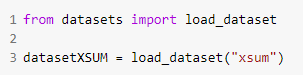
\includegraphics[scale=1]{SnippetXsum.png}
\end{center}
\subsubsection{\textit{Dataset} OrangeSum}
$ _{} $ $ _{} $ $ _{} $ $ _{} $ $ _{} $Ces données sont introduites à travers l'article \cite{eddine2020barthez} et ont été constituées en récupérant les contenus du site Web \textbf{Orange Actu}\footnote{\href{https://actu.orange.fr/}{https://actu.orange.fr/}}. Les pages scrappées couvrent presque une décennie, de février 2011 à septembre 2020. Elles appartiennent à cinq catégories prin\-ci\-pa\-les : France, monde, politique, automobile, et société . La catégorie société est elle-même divisée en 8 sous-catégories : santé, environnement, people, culture, médias, high-tech, insolite, et divers. Ce jeu de données est considéré comme l'équivalent en langue française du jeu de données \textit{XSum} en ce qui concerne le degré d'abstraction des résumés.\\
Pour ce mémoire, nous avons utilisé les données \textit{OrangeSum} tel que retrouvées sur le point d'entrée \textbf{GEM/OrangeSum} \footnote{\href{https://huggingface.co/datasets/GEM/OrangeSum}{https://huggingface.co/datasets/GEM/OrangeSum}}. Il peut donc être chargé identiquement que les 2 jeux de données précédents, \textit{XSum} et \textit{CNN/DailyMail}, en utilisant le nom de checkpoint \textit{GEM/OrangeSum}.
\subsubsection{\textit{Dataset} for-ULPGL-Dissertation}
Le jeu des données que nous avons dénommé \textbf{for-ULPGL-Dissertation} a été constitué par nous, à partir du sous-ensemble dénommé  \textit{abstract} du \textit{dataset} \textit{OrangeSum} mentionné dans la sous section précédente. Les données d'\textit{OrangeSum-Abstract} peuvent être chargées avec python en utilisant :
\begin{center}
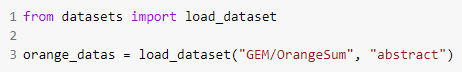
\includegraphics[scale=1]{SnippetOrangeAbstract.PNG}
\end{center}
A ces données, nous avons ajouté les quelques résumés jusque là générés grâce à notre système (dénommé \textbf{Mon Résumeur}). Plus exactement, la version actuelle (version $ 0.0.1 $ du $ 15/10/2022 $) de ce \textit{dataset} est constituée de $ 24 401 $ données en provenance d'\textit{OrangeSum-Abstract} et $ 450 $ données en provenance de \textbf{Mon Résumeur}. Soit environs $ 2\% $ du total en provenance de \textbf{Mon Résumeur}.\\
Nous ferons constamment évoluer ce \textit{dataset}, avec l'augmentation des résumés générés par notre système, de manière à ce qu'il soit ma\-jo\-ri\-tai\-re\-ment constitué des données jugées \textit{bonnes} par les utilisateurs de notre système.\\
Nous avons \textit{uploadé} le \textit{dataset} ainsi constitué dans notre compte \textit{hugging face}. Il y est pu\-bli\-que\-ment accessible et on peut y voir tous les détails sup\-plé\-men\-tai\-res \footnote{\href{https://huggingface.co/datasets/krm/for-ULPGL-Dissertation}{https://huggingface.co/datasets/krm/for-ULPGL-Dissertation}}. Comme il est au point d'entrée \textbf{krm/for-ULPGL-Dissertation}, on peut le charger avec \textit{Python} grâce aux bouts de code :
\begin{center}
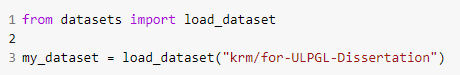
\includegraphics[scale=1]{SnippetMyDataset.PNG}
\end{center}

\subsection{Modèles utilisés pour la synthèse abstractive}
\subsubsection{Modèle BART optimisé}
$ _{} $ $ _{} $ $ _{} $ $ _{} $ $ _{} $Le modèle \textit{BART} \cite{BART} est celui que nous avons choisi comme modèle principal pour la synthèse abstractive dans notre système. Son objectif de pré-entraînement est assez général pour former un excellent modèle de langue comme nous l'avons décrit au chapitre précédent (voir le point \ref{BARTmodel}). Vu que notre système est destiné à fonctionner en production et non pas uniquement dans le monde de la recherche, il nous a été important de choisir une déclinaison de ce modèle adaptée à nos fins. C'est pour cela que nous avons choisi, pour notre système, d'utiliser la déclinaison accessible au \textit{checkpoint} \textbf{sshleifer/distilbart-cnn-12-6} finetuné pour la synthèse des textes. Ce \textit{transformer} peut être chargé très sim\-ple\-ment en utilisant le \textit{pipeline} traditionnel disponibilisé sur \textit{Hugging Face}\footnote{\href{https://huggingface.co/sshleifer/distilbart-cnn-12-6}{https://huggingface.co/sshleifer/distilbart-cnn-12-6}} par son auteur mais ce n'est pas très optimal de s'y prendre comme cela. C'est la raison pour laquelle, nous avons implémenté un \textit{pipeline} (comme on peut le voir sur la figure \ref{PipelineSumm}) nous permettant d'utiliser ce modèle de façon optimale, sans augmenter la complexité de calcul associée aux têtes d'attention de tous les modèles du type \textit{transformer} \cite{vaswani2017attention}. Les justifications des choix d'implémentation sont données au dernier point de ce chapitre.\\
Il faut noter que ce modèle est prévu exclusivement pour la langue anglaise.
\subsubsection{Modèle BARThez}
$ _{} $ $ _{} $ $ _{} $ $ _{} $ $ _{} $Le modèle \textit{BARThez} \cite{eddine2020barthez} est un modèle pré-entraîné sur du texte en français. Pour la synthèse abstractive, nous avons utilisé sa déclinaison finetunée sur le dataset \textit{OrangeSum} et disponible au \textit{checkpoint} \textbf{moussaKam/barthez-orangesum-abstract}. Néanmoins, on ne peut pas se contenter de ce modèle pour la synthèse en langue française car, étant donné le \textit{dataset} sur lequel il a été entraîné, la qualité de ses résumés n'est pas très satisfaisante quand on veut l'utiliser pour la production des résumés génériques sur des documents du type narratif et littéraire comme on le voudrait pour un système à usage général. En plus l'une des ses limitations est qu'il a une grande tendance à attribuer les propos des textes du résumé aux personnalités publiques actuelles quand bien même elles n'apparaissent pas dans le texte source (biais introduit par son \textit{dataset}). Les objectifs de pré-entraînement sont similaires à ceux du modèle \textit{BART}, donc il s'agit bien d'un modèle du type \textit{BART}. 
\subsubsection{Modèle mBARThez}
$ _{} $ $ _{} $ $ _{} $ $ _{} $ $ _{} $Le modèle \textit{mBARThez} est un modèle introduit dans l'article \cite{eddine2020barthez} (le même que celui de \textit{BARThez}) et basé sur \textbf{mBART}. Il s'agit d'un modèle pré-entraîné sur plusieurs langues et entraîné juste à prédire les mots masqués dans un texte. Nous l'avons finetuné pour pouvoir l'utiliser pour la synthèse automatique et espérer corriger avec le temps les faiblesses du modèle \textit{BARThez}. Pour le \textit{finetuning}, nous sommes parti du modèle \textit{mBARThez} re\-trou\-va\-ble au \textit{checkpoint} \textbf{moussaKam/mbarthez} \footnote{\href{https://huggingface.co/moussaKam/mbarthez}{https://huggingface.co/moussaKam/mbarthez}}.\\
Après entraînement de \textit{mBARThez}, nous avons produit un modèle pouvant être utilisé pour la synthèse (nous l'avons dénommé \textbf{BARTkrame-abstract}). 
\subsubsection{Modèle BARTkrame-abstract}
$ _{} $ $ _{} $ $ _{} $ $ _{} $ $ _{} $Il s'agit d'un modèle obtenu par \textit{finetuning} de \textit{mBARThez} sur notre \textit{dataset} dénommé \textit{for-ULPGL-Dissertation}. Cela nous a permis d'obtenir le \textit{checkpoint} \textbf{krm/BARTkrame-abstract} dont tous les détails sont accessibles sur la plateforme \textit{Hugging Face} où nous l'avons \textit{uploadé} \footnote{\href{https://huggingface.co/krm/BARTkrame-abstract}{https://huggingface.co/krm/BARTkrame-abstract}}.\\
$ _{} $ $ _{} $ $ _{} $ $ _{} $ $ _{} $En terme d'architecture, il s'agit d'un \textit{transformer} du type \textit{BART}, de même architecture que \textit{mBART}\cite{mBART_liu2020multilingual} car c'est ce qui a été utilisé comme modèle de base pour produire \textit{mBARThez} que nous avons finetuné enfin pour obtenir \textit{BARTkrame-abstract}.\\
C'est-à-dire qu'il s'agit d'un \textit{transformer} d'architecture exactement similaire à celle proposée à l'initial par \textit{Vaswani et al.} \cite{vaswani2017attention}  constitué de $ 12 $ couches dans l'encodeur et $ 12 $ dans le décodeur avec une dimension de $ 1024 $ \textit{tokens} pour le vecteur caché, sur $ 16 $ têtes d'attention.
\subsubsection{Modèle Pegasus}
$ _{} $ $ _{} $ $ _{} $ $ _{} $ $ _{} $Il s'agit de l'un des modèles jugés les plus performants pour les tâches de synthèse abstractive \cite{PEGASUSzhang2020pegasus}. En effet, son objectif de pré-entraînement est très proche d'une tâche de synthèse. Néanmoins, nous avons fini par le supprimer des modèles que nous rendons accessibles à travers notre \textit{API} à cause de sa lenteur et de sa taille. Cela est dû au fait que, du point de vu qualitatif, l'abstraction est parfois poussée trop loin de telle sorte que ce qui est dans la synthèse ne correspond pas vraiment à l'idée véhiculée par le texte source, le rapprochant beaucoup plus des systèmes de génération automatique des textes. Pour tirer ces conclusions, nous nous sommes servi du \textit{checkpoint} dénommé \textbf{google/pegasus-xsum} \footnote{\href{https://huggingface.co/google/pegasus-xsum}{https://huggingface.co/google/pegasus-xsum}}.
\subsection{Tests}
$ _{} $ $ _{} $ $ _{} $ $ _{} $ $ _{} $Nous avons mené plusieurs tests, à la fois sur les modèles abstractifs et sur les algorithmes de synthèse extractive de notre système. Les tests avaient pour objectif de démontrer le bien-fondé des techniques que nous avons choisi pour la synthèse automatique.\\
Nous avons utilisé comme métriques d'évaluation les mesures \textit{ROUGE-1}, \textit{ROUGE-2}, \textit{ROUGE-L} et une variante de cette dernière dénommée \textit{ROUGE-LSum} car il s'agit de loin des mesures les plus utilisées en synthèse automatique \cite{MaaliMnasri}.
\subsubsection{Tests sur les algorithmes de synthèse extractive}
$ _{} $ $ _{} $ $ _{} $ $ _{} $ $ _{} $Ce test a deux principaux objectifs :
\begin{itemize}
\item[-] choisir les poids à affecter aux divers algorithmes qui forment le système \textit{merging} (\ref{ArchiGlobExtract}).
\item[-] établir une mesure des performances de la partie qui fonctionne par combinaison des divers algorithmes de synthèse extractive (voir la figure \ref{ArchiGlobExtract} qui représente le système en question que nous avons nommé \textit{merging}) par rapport au module python dédié à la synthèse extractive, module dénommé \textit{gensim} (choisi principalement pour sa rapidité);
\end{itemize}
Le test a été effectué en se servant de $ 2 $ \textit{datasets} bien connus en synthèse automatique, à savoir \textit{CCN / DailyMail} et \textit{XSum}. Ce test a été mené en anglais pour ne pas avoir à traduire les \textit{datasets} et ainsi avoir des résultats les plus authentiques possible. Pour chacun de ces \textit{datasets}, nous avons réalisé nos expérimentations sur les données de test. Nous avons choisi ces deux \textit{datasets} car ils sont en quelques sortes complémentaires. En effet, \textit{CCN / DailyMail} est essentiellement extractif tandis que \textit{XSum} est beaucoup plus abstractif \cite{eddine2020barthez}.
\subsubsection{Tests sur BART et BART optimisé}
$ _{} $ $ _{} $ $ _{} $ $ _{} $ $ _{} $Ce test avait pour objectif d'évaluer les performances du modèle \textit{BART} quand on l'utilise à travers le pipeline implémenté par nous selon la figure \ref{PipelineSumm} par rapport à une utilisation classique (selon le pipeline classique \cite{GRAAL_HF_tunstall2022natural}). Nous avons pour cela utilisé les \textit{datasets}
\textit{CCN / DailyMail} et \textit{XSum} sur le \textit{checkpoint} dénommé \textit{sshleifer/distilbart-cnn-12-6} que nous avons utilisé comme modèle \textit{BART} dans l'ensemble du système. 
\subsubsection{Précisions sur l'entraînement et les tests de BARTKrame-abstract}
$ _{} $ $ _{} $ $ _{} $ $ _{} $ $ _{} $La version actuelle de ce modèle (le $ 16/10/2022 $, version $ 0.0.1 $) a été obtenue après entraînement de \textit{mBARThez} avec \textbf{$  5000 $ données d'entraînement et $ 100 $ données de validation} provenant du \textit{dataset} \textit{for-ULPGL-Dissertation} (le nombre de données a été réduit suite aux limitations en terme de ressources matérielles dont nous disposions). Nous avons utilisé, pour cet entraînement, un environnement sur \textit{google colab}\footnote{\href{https://colab.research.google.com/}{https://colab.research.google.com/}} équipé d'un \textit{GPU} et à présent l'entraînement a été fait sur $ 12 $ époques et a duré $ 8 $ heures. Les hy\-per\-pa\-ra\-mè\-tres utilisés peuvent être ainsi présentés :
\begin{itemize}
\item[•] \textit{Learning rate initial :} $ 5.6*10^{-6} $;
\item[•] Taille des batchs (\textit{batch size}) : 4;
\item[•] Optimiseur : \textit{Adam} (avec $ \beta = 0.999 $ et $ \epsilon = 1*10^{-8} $)
\item[•] Le \textit{Learning rate} était à décroissance linéaire;
\item[•] Le grain de sélection aléatoire des données était de $ 42 $;
\item[•] Métrique : \textit{ROUGE}.
\end{itemize}
Pour plus d'informations sur notre modèle et le processus d'entraînement, se rapporter à son dépôt sur \textit{Hugging Face}\footnote{\href{https://huggingface.co/krm/BARTkrame-abstract}{https://huggingface.co/krm/BARTkrame-abstract}}.\\
Le test réalisés sur ce modèle ont été faits sur le dataset \textit{for-ULPGL-Dissertation} car notre objectif est d'obtenir un modèle principalement en français. Une partie des résultats de test a été obtenue immédiatement après entraînement (c'est-à-dire sur les données de validation) et nous avons réalisé après cela un autre test sur les données de test de notre \textit{dataset}.

\subsection{Résultats des tests}
Pour ces résultats, il faut noter que plus une mesure est supérieure, plus le modèle a de chance de donner des résultats de bonne qualité. Ce n'est pas toujours le cas mais la mesure \textit{ROUGE} ici utilisée est un excellent indicateur des performances d'un système de résumé automatique (voir la section \ref{sectionSurROUGE}).
\subsubsection{Algorithmes de synthèse extractive}
\begin{itemize}
\item[1°)] \textbf{Recherche des poids des modèles constituant \textit{merging}}\\
Pour cet essai, il nous a d'abord fallu évaluer la confiance que nous pouvons accorder à chaque modèle constituant \textit{merging}. Ce que nous appelons \textit{merging} est formé, comme on peut le voir sur la figure \ref{ArchiGlobExtract} par les algorithmes de synthèse extractive suivants : \textit{TF-IDF}, \textit{LSA}, \textit{Heuristiques}, \textit{TextRank}, \textit{LexRank} et \textit{Luhn}. Pour la recherche des poids, nous avons considéré uniquement les résultats des tests sur le \textit{dataset} \textit{CNN/DailyMail} car il est plus adapté à la synthèse extractive. Les résultats ont été les suivants :
\begin{center}
\captionof{table}{Résultats ROUGE des algorithmes de \textit{merging} sur \textit{CNN/DailyMail}}
\label{SumyOnCnn}
\setlength{\arrayrulewidth}{1pt}
\definecolor{gris}{gray}{0.65}
\begin{tabular}{|p{4cm}||p{2.5cm}|p{2.5cm}|p{2.5cm}|p{2.5cm}|}
\hline
\cellcolor{gris}\textbf{Algorithmes} & R-1  & R-2 & R-L & R-LSum \\
\hline
\hline
\textbf{Heuristique} & $ 24.72 $  & $ 7.95 $  & $ 16.44 $ & $ 19.64 $ \\
\hline
\textbf{LexRank} & $ 22.88 $ & $ 5.88 $  & $ 15.02 $ & $ 18 $ \\
\hline
\textbf{TextRank} & $ 19.91 $ & $ 5.06 $ & $ 13.52 $ & $ 16.13 $ \\
\hline
\textbf{LSA} & $ 20.43 $ & $ 3.68 $ & $ 12.84 $ & $ 15.70 $ \\
\hline
\textbf{Luhn} & $ 19.66 $ & $ 4.79 $ & $ 12.66 $ & $ 15.39 $ \\
\hline
\textbf{Tf-Idf} & $ 10.98 $ & $ 1.99 $ & $ 7.77 $ & $ 8.95 $ \\
\hline
\end{tabular}
\end{center}
Pour la recherche des poids, nous avons appliqué une méthode heuristique simple. En vertu des résultats que nous avons dans le tableau \ref{SumyOnCnn}, nous avons accordé les scores $ 1 $, $ 2 $, $ 3 $, $ 4 $, $ 5 $ et $ 6 $ respectivement aux algorithmes \textit{Tf-Idf}, \textit{Luhn}, \textit{LSA}, \textit{TextRank}, \textit{LexRank} et \textit{Heuristique} comme ils se suivent dans le tableau. Ensuite, nous avons normalisé ces poids en appliquant une fonction \textit{softmax} à cet ensemble de rangs. Donc, en appliquant $ e^{i}/\left( \sum_{n=1}^{6} e^{n}\right) $ pour tout $ i\in \left\lbrace 1, 2, 3, 4, 5, 6\right\rbrace $ nous avons trouvé les poids suivants :\newpage
\begin{center}
\captionof{table}{Poids des algorithmes constituant \textit{merging}}
\label{MergingWeights}
\setlength{\arrayrulewidth}{1pt}
\definecolor{gris}{gray}{0.65}
\begin{tabular}{|p{2.4cm}|p{2.4cm}|p{2.4cm}|p{2.4cm}|p{2.4cm}|p{2.4cm}|}
\hline
 \textbf{Heuristique} & \textbf{LexRank}  & \textbf{TextRank} & \textbf{LSA} & \textbf{Luhn}  & \textbf{Tf-Idf} \\
\hline
\hline
 0.633 & 0.233  & 0.0857 & 0.0315 & 0.0116  & 0.0042 \\
\hline
\end{tabular}
\end{center}
\item[2°)] \textbf{Comparaison quantitative de Merging avec Gensim}\\
L'évaluation de ces deux modèles sur \textit{CNN/DailyMail}, en se servant des poids listés dans le tableau \ref{MergingWeights}, a donné les résultats suivants :
\begin{center}
\captionof{table}{Comparaison des algorithmes Gensim et \textit{merging} sur \textit{CNN/DailyMail}}
\label{MergingVsGensimOnCNN}
\setlength{\arrayrulewidth}{1pt}
\definecolor{gris}{gray}{0.65}
\begin{tabular}{|p{4cm}||p{2.5cm}|p{2.5cm}|p{2.5cm}|p{2.5cm}|}
\hline
\cellcolor{gris}\textbf{Algorithmes} & R-1  & R-2 & R-L & R-LSum \\
\hline
\hline
\textbf{Gensim} & $ 31.74 $  & $ 12.28 $  & $ 20.69 $ & $ 27.70 $ \\
\hline
\textbf{Merging} & $ 23.19 $ & $ 6.70 $  & $ 15.05 $ & $ 18.17 $ \\
\hline
\end{tabular}
\end{center}
L'évaluation de ces deux modèles sur \textit{XSum}, en se servant des poids listés dans le tableau \ref{MergingWeights}, a quant à elle donné les résultats suivants :
\begin{center}
\captionof{table}{Comparaison des algorithmes Gensim et \textit{merging} sur \textit{XSum}}
\label{MergingVsGensimOnXSum}
\setlength{\arrayrulewidth}{1pt}
\definecolor{gris}{gray}{0.65}
\begin{tabular}{|p{4cm}||p{2.5cm}|p{2.5cm}|p{2.5cm}|p{2.5cm}|}
\hline
\cellcolor{gris}\textbf{Algorithmes} & R-1  & R-2 & R-L & R-LSum \\
\hline
\hline
\textbf{Gensim} & $ 15.10 $  & $ 2.50 $  & $ 10.13 $ & $ 11.29 $ \\
\hline
\textbf{Merging} & $ 14.90 $ & $ 1.88 $  & $ 10.09 $ & $ 10.12 $ \\
\hline
\end{tabular}
\end{center}
\end{itemize}
\subsubsection{Résultats de BART en usage normal puis en usage optimisé}
Les tests sur le jeu des données \textit{CNN/DailyMail} ont donné les résultats suivants :
\begin{center}
\captionof{table}{Comparaison de BART avec BART optimisé sur \textit{CNN/DailyMail}}
\label{BARTvsBARToptCNN}
\setlength{\arrayrulewidth}{1pt}
\definecolor{gris}{gray}{0.65}
\begin{tabular}{|p{5cm}||p{2.5cm}|p{2.5cm}|p{2.5cm}|p{2.5cm}|}
\hline
\cellcolor{gris}\textbf{Algorithmes} & R-1  & R-2 & R-L & R-LSum \\
\hline
\hline
\textbf{BART optim.} & $ 43.72 $  & $ 20.22 $  & $ 30.06 $ & $ 36.62 $ \\
\hline
\textbf{BART normal} & $ 36.66 $ & $ 14.31 $  & $ 25.88 $ & $ 31.038 $ \\
\hline
\end{tabular}
\end{center}
Et les tests sur le jeu des données \textit{XSum} ont donné :
\begin{center}
\captionof{table}{Comparaison de BART avec BART optimisé sur \textit{XSum}}
\label{BARTvsBARToptXSum}
\setlength{\arrayrulewidth}{1pt}
\definecolor{gris}{gray}{0.65}
\begin{tabular}{|p{5cm}||p{2.5cm}|p{2.5cm}|p{2.5cm}|p{2.5cm}|}
\hline
\cellcolor{gris}\textbf{Algorithmes} & R-1  & R-2 & R-L & R-LSum \\
\hline
\hline
\textbf{BART optim.} & $ 20.57 $  & $ 3.50 $  & $ 13.42 $ & $ 13.41 $ \\
\hline
\textbf{BART normal} & $ 17.67 $ & $ 2.66 $  & $ 12.08 $ & $ 12.091 $ \\
\hline
\end{tabular}
\end{center}

\subsubsection{Résultats des tests de BARTKrame-abstract}
Les tests sur le jeu des données \textit{for-ULPGL-Dissertation} ont donné les résultats suivants:
\begin{center}
\captionof{table}{Résultats de test de \textit{BARTkrame-abstract} sur \textit{for-ULPGL-Dissertation} }
\label{ResultBARTkrame-abstract}
\setlength{\arrayrulewidth}{1pt}
\definecolor{gris}{gray}{0.65}
\begin{tabular}{|p{5cm}||p{2.5cm}|p{2.5cm}|p{2.5cm}|p{2.5cm}|}
\hline
\cellcolor{gris}\textbf{Données} & R-1  & R-2 & R-L & R-LSum \\
\hline
\hline
\textbf{Validation} & $ 27.03 $  & $ 13.34 $  & $ 23.92 $ & $ 24.19 $ \\
\hline
\textbf{Test} & $ 24.08 $ & $ 7.28 $  & $ 19.30 $ & $ 19.29 $ \\
\hline
\end{tabular}
\end{center}

\textbf{Il faudra noter que le dataset utilisé pour entraîner ce modèle, ainsi que le modèle lui-même, seront entrain d'être améliorés. Pour avoir les résultats actualisés au-delà de la date de soumission de ce document, il faut se rapporter à leurs liens (dépôts HuggingFace sus-mentionnés pour \textit{BARTkrame-abstract} et pour \textit{for-ULPGL-Dissertation}).}
\subsection{Interprétation des résultats}
\subsubsection{Système de synthèse extractive}
$ _{} $ $ _{} $ $ _{} $ $ _{} $ $ _{} $Comme on peut le voir dans les tableaux \ref{MergingVsGensimOnCNN} et \ref{MergingVsGensimOnXSum}, les performances du module python \textit{gensim} demeurent supérieures à celles de \textit{merging}. Cela est un fait, du point de vu quantitatif. Néanmoins, comme pourra en juger le lecteur au vu des exemples mis en annexe, cela n'est pas complètement vrai du point de vu qualitatif.\\
$ _{} $ $ _{} $ $ _{} $ $ _{} $ $ _{} $En effet, le modèle \textit{merging} tel que nous l'avons implémenté gère mieux le ratio entré par l'utilisateur et est moins sensible aux problèmes introduits par les sauts de ligne arbitraires dans le texte. Également, \textit{merging} repère très bien les éléments saillants du texte (voir l'annexe \ref{AnnexesExemples}) .\\
$ _{} $ $ _{} $ $ _{} $ $ _{} $ $ _{} $Il faut finalement constater que les mesures sur \textit{XSum} sont toujours inférieures à celles faites sur \textit{CNN/DailyMail}. Cela est très normal et justifié par le fait que le \textit{dataset} \textit{CNN/DailyMail} est essentiellement du type extractif alors que \textit{XSum} est du type \textit{abstractif}.
\subsubsection{BART et BART optimisé}
$ _{} $ $ _{} $ $ _{} $ $ _{} $ $ _{} $Comme on peut le voir au travers des tableaux \ref{BARTvsBARToptCNN} et \ref{BARTvsBARToptXSum}, les résultats obtenus avec le modèle \textit{BART} en usage optimal sont largement supérieurs à ceux obtenus en usage classique (normale). Le test sur \textit{CNN/DailyMail} donne des résultats sans équivoque sur la supériorité de \textit{BART optimisé} par rapport au \textit{BART classique}. Néanmoins, les résultats sur \textit{XSum} sont proches (comme on le voit dans le tableau \ref{BARTvsBARToptXSum}) et cela est bien évident car, comme \textit{XSum} est formé des résumés à tendance plus abstraite et que le modèle \textit{BART} est la base de ces deux implémentations (classique et optimisée), aucune ne devait dépasser un certain seuil en ce qui concerne la ressemblance à \textit{XSum}. En plus, la mesure \textit{ROUGE} est incapable de repérer les similarités sémantiques quand des tournures différentes sont utilisées. Néanmoins, l'utilisation de la mesure \textit{ROUGE} sur un \textit{dataset} à tendance abstractive est un bon indicateur de la fidélité du modèle au texte d'origine quand il s'agit d'un modèle abstractif.
\subsubsection{Commentaires sur les résultats de BARTkrame-abstract}
$ _{} $ $ _{} $ $ _{} $ $ _{} $ $ _{} $Les résultats obtenus sur \textit{BARTkrame-abstract} ne devaient pas différer assez sur les données de validation par rapport aux données de test car les données proviennent d'un même \textit{dataset} et, comme le \textit{dataset} a été constitué par un choix aléatoire des données à affecter aux différentes catégories (\textit{train}, \textit{test} et \textit{validation}), les caractéristiques statistiques des données de validation sont approximativement les mêmes que celles des données de test. Cela devait suffire pour assurer que les résultats obtenus sur les données de test et ceux obtenus sur les données de validation soient assez proches.\\
$ _{} $ $ _{} $ $ _{} $ $ _{} $ $ _{} $La signification des résultats du tableau \ref{ResultBARTkrame-abstract} est simplement que le modèle est encore très sensible à des petites variations. Donc il n'est pas encore stable et l'entraînement doit être poursuivi. Cela est évidemment clair quand on regarde les résultats qualitatifs (les synthèses) obtenus en utilisant ce modèle dans notre système. On peut voir en effet que le modèle parvient à capturer les points importants mais ne parvient pas encore à repérer clairement où s'arrêter, voir l'annexe \ref{AnnexesExemples}.

\section{Justification des choix d'implémentation}
$ _{} $ $ _{} $ $ _{} $ $ _{} $ $ _{} $Voici donc quelques justifications très sommaires des choix d'implémentation que nous avons faits. Les points saillants sont principalement ici présentés :
\begin{itemize}
\item[•] L'un des modules utilisés pour la synthèse extractive est \textit{gensim}. Nous l'avons prin\-ci\-pa\-le\-ment choisi comme algorithme de base de la synthèse extractive suite à sa rapidité. Il implémente néanmoins l'algorithme \textit{Tf-Idf} avec quelques optimisations \cite{srinivasaGENSIMnatural}.
\item[•] Pour le module mélangeant un grand nombre d'algorithmes utilisés pour la synthèse extractive, nous avons opté pour cette approche car nous sommes partis de l'idée selon laquelle, du point de vu qualitatif, une synthèse qui serait générée en prenant en compte divers aspects serait plus susceptible d'être riche que les autres. Bien que les résultats quantitatifs (mesure \textit{ROUGE}) n'ont pas été très satisfaisants, nous estimons avoir eu raison d'implémenter ces algorithmes au vu de la valeur ajoutée en terme qualitatif comme on peut en juger grâce aux synthèses mises à l'annexe \ref{AnnexesExemples}.
\item[•] Pour la synthèse abstractive, le fait de tourner notre choix vers les modèles du type \textit{BART} a été inspiré par la nécessité de réaliser des synthèses abstraites mais pas trop pour ne pas s'éloigner du contenu du texte source. Cela nous a amené à exclure \textit{PEGASUS} bien que ce soit l'un des modèles les mieux cotés en synthèse abstractive. En fait, \textit{PEGASUS} s'éloigne souvent des vraies idées véhiculées par le texte source. En plus, étant donné que le modèle \textit{BART} est moins pesant et plus manipulable que le modèle \textit{T5}, il a été l'unique à considérer (comme \textit{PEGASUS} et \textit{T5} étaient \textit{ipso facto} exclus).
\item[•] Comme point de repère avec les modèles complètement conçus en français, nous avons utilisé \textit{BARThez} car c'est la référence française en ce qui concerne les \textit{tranformers} de type encodeur-décodeur.
\item[•] Pour l'entraînement de notre modèle, nous sommes parti de \textit{mBARThez} qui est à la base un modèle \textit{mBART} dont le pré-entraînement a été poursuivi en insérant une grande masse des données en français \cite{eddine2020barthez}. Comme nous devions réaliser le \textit{finetuning} sur du texte en français pour obtenir un modèle complètement en français, nous estimons que c'est l'approche la plus appropriée et devant nous permettre de partir d'un modèle de langue déjà très bon en français. Ce dernier fait a pour avantage de nous permettre de diminuer les données d'entraînement.
\item[•] Pour l'implémentation de l'\textit{API}, nous avons choisi d'utiliser \textit{Flask} étant donné qu'il donne une grande liberté aux développeurs. Il n'a pas une structure préconçue et imposante.
\item[•] L'utilisation de \textit{ReactJS} pour la partie client a été motivée par sa popularité, mais également nous nous sentons plus à l'aise avec la syntaxe et l'architecture de ce \textit{framework}.
\item[•] Concernant le fait de réaliser une \textit{API} parfaitement distinguée, l'objectif est de permettre l'implémentation, par divers développeurs, de toute forme de systèmes pouvant en utiliser les services, participant par la même occasion à l'amélioration de notre modèle de synthèse. C'est d'ailleurs la raison pour laquelle nous avons également donné aux utilisateurs la possibilité d'évaluer les résumés qu'ils obtiennent. Cela constituera en fait un écosystème d'annotation des résumés par des humains.
\end{itemize}
\section{Conclusion partielle}
$ _{} $ $ _{} $ $ _{} $ $ _{} $ $ _{} $Dans ce chapitre, qui est le dernier de notre travail, nous venons de finaliser la conception de notre système. Cela nous a permis de montrer que le système a une ar\-chi\-tec\-tu\-re \textit{3-tiers} classique, avec une petite base des données qui nous permet également de récolter les données de synthèse pouvant par la suite s'utiliser pour améliorer les modèles de \textit{machine learning} dédiés à la synthèse automatique des documents.\\
Nous y avons également présenté les diverses métriques couramment utilisées pour l'é\-va\-lua\-tion des systèmes de synthèse automatique, tout en utilisant le paquet \textit{ROUGE} qui est la métrique la plus utilisée pour cette fin.\\
$ _{} $ $ _{} $ $ _{} $ $ _{} $ $ _{} $Ce chapitre nous a non seulement permis de décrire complètement l'implémentation de notre système mais également, il nous a permis de montrer que le modèle \textit{BART} tel que nous l'avons utilisé pour la synthèse abstractive est plus performant que si on l'utilisait dans une pipeline classique. Nous avons également montré que les résultats du module \textit{gensim} pour la synthèse automatique sont meilleurs que ceux de l'algorithme \textit{merging}, mais que ce dernier est qua\-li\-ta\-ti\-ve\-ment très satisfaisant et plus robuste aux variations mineures dans les textes. Nous avons également montré que le modèle \textit{BARTkrame-abstract}, qui a été obtenu après \textit{finetuning} de \textit{mBARThez} (un modèle basé sur \textit{mBART}) sera entrain d'être amélioré au fil de l'utilisation du système, étant donné que tout l'ensemble a été conçu en tenant compte de cet aspect.